\chapter{Monte Carlo simulation}

\begin{overview}
  Monte Carlo simulation entails running a deterministic simulation
  many times with variables chosen from the correct distributions.
  For valid results, the random numbers must be generated correctly,
  the simulation run correctly and the results collected with correct
  calculation of the output distributions.  This chapter explores
  these aspects of Monte Carlo simulation.
\end{overview}

\section{Introduction}
Monte Carlo simulation is the brute-force algorithm of the statistical world. At
the heart of the method is the idea that it is often much easier to develop a
high-fidelity deterministic model of a process than characterising a stochastic
process.  Using these deterministic models, one can estimate the distribution of
output variables using input variables generated to conform to a known input
distribution.  For this process to work, we need realistic inputs, a good
deterministic model and a reliable way of interpreting the results.

% FIXME: We need a nice figure here illustrating the concept and a better
% reference than moody

\section{Input generation}
Within the context of MC simulation, ``inputs'' are sources of variance. Variance
can be characterised as ``real'' variance, or external variance and uncertainty,
which is inherent in the model, but does not exist in the real
process\footnote{We assume here that deterministic models are able to capture the
process behaviour}.  In a sense, the variability of the inputs captures our
uncertainty about their behaviour.  We therefore distinguish between  varibles 
that remain fixed during a simulation, but could assume different values for any
given simulation, and those that would be expected to assume many values over a
given simulation time.  In the first case we simply have to generate values
conforming to a known distribution.  In the first case, we need to generate
realistic input sequences, typically including  realistic transitions between the
different values they attain.

% FIXME: Create a figure showing the taxonamy of variables.

\section{Pseudo-random number generation}
As modern computers are deterministic devices, it is theoretically
impossible to use them to generate a sequence of truly random numbers
\citehere.  However, it is possible to generate a (periodic) sequence
of numbers that are not significantly different from a random number
sequence.  Such a sequence is termed pseudo-random.

One of the more active researchers in the field, George Marsaglia, has
proposed several popular schemes for generating such sequences.\citehere

\subsection{Uniformly distributed}
The most commonly used distribution for RNGs is the uniform distribution. 
Numbers are usually generated in the range of $[0, N)]$ where $N$ is some large
number.  Continuously distributed values in the range $[0,1]$ are generated from
the discrete variable by dividing  by  $N$. The most popular generators are the
congruential generators.



Marsaglia suggests the use of XOR-based generators for normal
applications where efficiency is important \citehere.

\subsection{Normally distributed}
Several routines exist to generate normally distributed pseudo-random
values.  Most of them involve drawing a number of uniformly
distributed values and manipulating them, but some purpose-built
algorithms exist~\citehere.

\subsection{Arbitrary distributions}
\subsubsection{Given a CDF}

\subsubsection{Given a number of bins}

\section{Sequence generation}
\subsection{Sequence probabilities}

\subsection{Markov chains}
A markov process can be described as a stochastic process posessing the
property that the probability of moving to a particular new state $i$ from an
old state $j$ is only dependant on $i$ and $j$, but not on the states that had
previously been attained.  It is common to express the probabilities of the
transitions in matrices as follows:
\begin{equation}
X = \left [ \begin{array}{cccc}
            p_{11} & p_{12}	& \ldots & p_{1n} \\
            & \vdots & \\
            p_{n1} & p_{n2} & \ldots & p_{nn}\\ 
            \end{array}\right]
\end{equation}

\section{Introduction}
A simulation is a reproduction under controlled circumstances of a
real-life situation.  The term has recently become strongly associated
with numeric evaluation of a computer model due to the increase in
speed and availability of computing resources.  This increase in speed
has led to much interest in stochastic simulation, where processes
with elements that are random are simulated.  An attractive branch of
stochastic simulation termed Monte Carlo simulation uses deterministic
models driven by stochastic input sequences to approximate the
distributions of output variables over time.  To do this, a good
deterministic model of the process is needed in addition to a good
method of generating realistic input sequences.

Correct input sequences are a prerequisite for reliable results from
stochastic simulation.  To generate them, the modeller must either
generate input sequences by hand, develop a model based on intuition
or understanding of the process, or use existing data.  Generating
input sequences by hand is a tedious and error-prone process and
intuition is not a particularly verifiable source of information.
This means that data-driven model development has been gaining favour
steadily as data becomes more accessible.

This chapter is covers three aspects of input signal generation:
First, the basic theory of Markov processes and hidden Markov models
is reviewed with a view on using them as generating processes for
input models. Second, signal segmentation is introduced.  This is the
first step in identifying state transition probabilities for discrete
Markov processes.  In this part, novel work done on the identification
of state transitions using multi-objective optimisation is introduced
and ideas for future research are posed. Third, the problem of
estimating state transition probabilities from the segmented signals
is discussed, touching on the issues that modellers should be aware
of.

Markov processes have featured strongly in stochastic sequence
identification and generation for many years, but some of the related
problems are still active research fields.

\section{Markov Processes}
\subsection{Discrete-time Markov Processes}
A stochastic process with state space $S$ has the Markov
property if the current state completely determines the probability of
the following state.  A sequence $X_1,X_2, \dots ,X_t$ having this
property is known as a Markov chain.

Stated mathematically, a Markov chain obeys the property
\begin{equation}
  \label{eq:markovproperty}
  \Pr(X_{t+1} = j|X_{t}=i) = \Pr(X_{m+1}=j|X_{m}=i)=p_{ij}
\end{equation}
in words, the probability that the next state will be equal to $j$ given
that the current state is $i$ is only dependant on the current state.

When $S$ is a countable set, the state transition probabilities can be written 
as a state transition matrix $P$ as shown for a 3 state process in
equation~\ref{eq:markovmatrix}
\begin{equation}
\label{eq:markovmatrix}
P = \left[ 
  \begin{array}{cccc}
    p_{11} & p_{12} & p_{13}\\
    p_{21} & p_{22} & p_{23}\\
    p_{31} & p_{32} & p_{33}\\
  \end{array} \right ]
\end{equation}

The probability of remaining within the state space must be unity,
hence we may write 
\begin{equation}
  \label{eq:rowsumone}
  \sum_{j\in S} p_{ij}=1~\forall~i \in S.
\end{equation}

Matrices with this property as well as the common-sense property
that $0 \leq p_{ij} \leq 1$ (as they are probabilities) are called
stochastic matrices.

The orientation of $P$ is not unique. The arrangement with the current
state in the rows and next state in the columns is known as a right
transition matrix. The transpose arrangement has also been used (see
for instance \citet{bhar_hidden_2004}) and is then described as a left
transition matrix. Modern engineering usage leans toward the
description used in this work.

A common way of visualising a Markov process with countable state
space is by showing a directed graph with the states in the nodes and
the transition probabilities on the edges as shown in
Figure~\ref{fig:markovgraph}. In these representations, it is
customary to neglect edges with zero probabilities.

\begin{figure}[htbp]
  \centering
  \begin{minipage}{0.4\textwidth}
    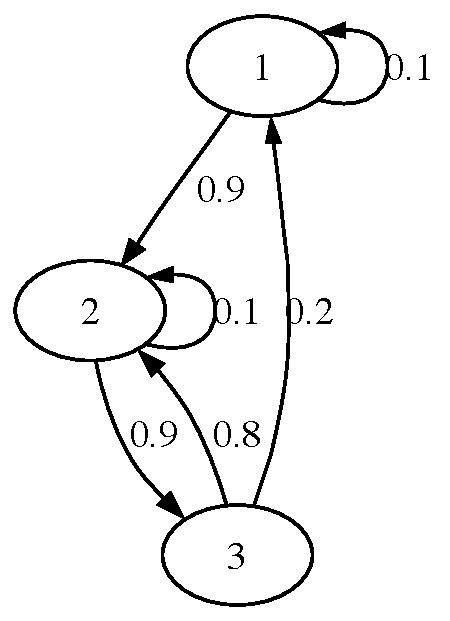
\includegraphics[scale=0.5]{smallmarkov}
  \end{minipage}
  \begin{minipage}{0.4\textwidth}
   $\displaystyle P = \left [ 
      \begin{array}{ccc} 
        0.1 & 0.9 & 0 \\ 
        0 & 0.1 & 0.9 \\ 
        0.2 & 0.8 & 0 
      \end{array} \right ]$
  \end{minipage}
  \caption{Markov process represented by a transition matrix and a graph}
  \label{fig:markovgraph}
\end{figure}

The state transition probabilities sufficiently describe the time
dependence of the process, but the initial state can not be determined
using the transition probabilities alone.  The probability of the
process starting out in a given state $i$ is denoted $\pi_i, i \in S$,
and the vector of initial state probabilities is called
$\vect{\pi}$. It can be seen that a discrete time Markov process
is completely described by its state space $S$, its state transition matrix
$P$ and its initial state probability vector $\vect{\pi}$.  If
$S$ is countable and has $N$ elements, $N^2 + N$ probabilities have to
be known to fully characterise the process.  For convenience, the
model is written $\lambda = (P, \vect{\pi})$.

\subsection{Hidden Markov Models} 
It is not always possible to observe the state (in the state space
$S$) of a Markov process directly. It may, however, be possible to
make observations from an observation space $O$ related to the state
of the process. If the probability of making a particular observation
is only related to the current state of the process, the process may
be described by a hidden Markov model (HMM). What is ``hidden'' in
this case are the true values of the Markov process states.

Figure~\ref{fig:hiddenmarkov} shows the situation graphically. If the
Markov process is in state 1, there are even odds that observation 2
or 3 will be made. In state 2, only observation 2 is made and state 3
is associated with observation 1 80\% of the time and observation 2
20\% of the time.

\begin{figure}[htbp]
  \centering
  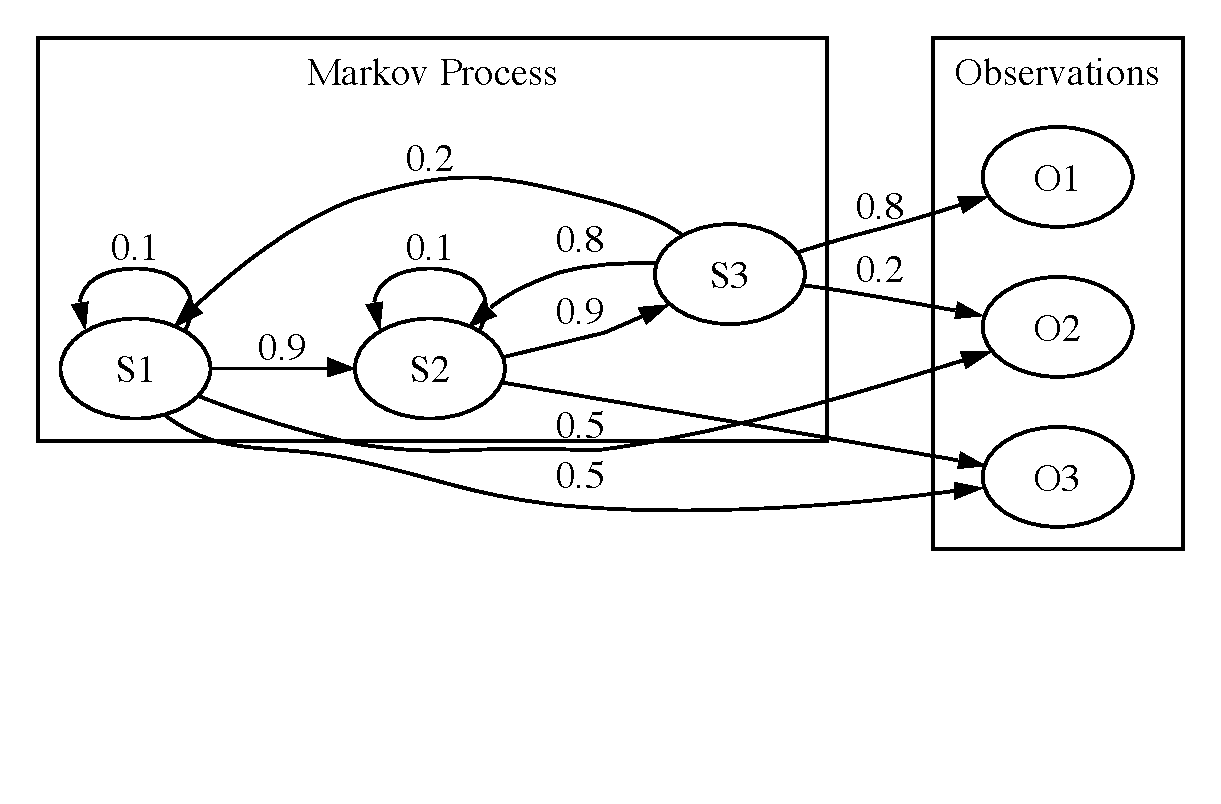
\includegraphics[scale=0.5,clip,trim=0 4cm 0 0]{smallhiddenmarkov}
  \caption{Graphical representation of a finite hidden Markov model}
  \label{fig:hiddenmarkov}
\end{figure}

The probabilities associated with a observation $k$ being made when
the process is in state $i$ may be written $b_{ik}$ and can be
arranged into an observation probability matrix $B$ in a similar
fashion as was previously done for $P$. One difference is that, while
$P$ was an $N \times N$ square matrix, $B$ will have $N$ rows
associated with the $N$ states of the Markov process and $M$ columns
associated with the observation space. An HMM as described here can
therefore be characterised by the same $N^2+N$ probabilities describing
the Markov process in addition to $MN$ observation probabilities.  The
model description can be abbreviated to $\lambda = (P, B, \vect{\pi})$.

There are three main problems associated with HMMs \citep{gamerman_markov_2006}:
\begin{itemize}
\item What is the probability of generating a specific output sequence
  from a particular model?
\item What is the most likely sequence of states that would lead to a
  particular output sequence?
\item How do we identify the model that corresponds to a given output
  sequence?
\end{itemize}

\subsection{Continuous-time Markov Processes}
The description of discrete-time Markov processes assumed that the
transition time was known or unimportant and one could imagine
simulating the process by picking a state $i$ and moving to the next
state with probability $p_{ij}$.  One shortcoming of such a
description is that there is no information about the amount of time a
process remains in a particular state before moving to the next (or
possibly same) state.  

% TODO: Flesh out this description
% look at perhaps http://www.stat.sfu.ca/~lockhart/richard/380/00_3/lectures/19/web.html
Continuous-time Markov processes encode the transition probabilities as
transition rates $q_{ij}$ (forming a $Q$ matrix as $p_{ij}$ formed a
$P$ matrix), such that
\begin{equation}
  \label{eq:contmarkov}
  \Pr(X(t+\Delta t) = j | X(t) = i) = 
  \begin{cases}
    1 - q_{ii}\Delta t + o(\Delta t) & \text{for } i = j \\
    q_{ij}\Delta t + o(\Delta t) & \text{otherwise}
  \end{cases}
\end{equation}

The idea is that, having changed to a particular state the probability of moving to the next one approaches one over time, but at different rates.


\subsection{Optimisation with variable numbers of events}
The optimisation methods discussed so far have a significant
disadvantage: it is not possible for them to choose the ``optimal''
number of segments as one of the design variables, as their design space
needs to have constant dimension. It is, however, possible to use
genetic algorithms (GAs) for this purpose, by using a crossover
operator allowing varying chromosome lengths.  One such operator is
the simple ``cut and splice'' operator, which chooses a crossover
point on the chromosome of each parent independently before exchanging
material.  The application of multi-objective GAs with varying
chromosome lengths may yield the first fully-automated optimisation
for fitting events, as it allows the number of events to be included
in the objective set.

Finding the Pareto-optimal set of fits in this way will enable much
richer analysis of time series.

\section{Estimating state transition probabilities}
The most direct method of estimating the state transition
probabilities of a Markov process is to count the number of
transitions in an input signal.  This strategy has some problems:
\begin{enumerate}
\item Certain transitions may not occur in the input signal, so that
  these transitions will never be simulated by the identified model
\item Segmentation of the input signal may bias the event types or
  transitions -- if a certain event is more often fit by the
  segmentation algorithm, that event will be over-represented in the
  transition matrix.
\end{enumerate}

If transitions between some events are very rare, it may be advisable
to introduce a small artificial probability into the matrix to ensure
that the event has a chance of  getting generated during the
simulation.  This is especially true if the repercussions of a certain
event combination are significant.  

Segmentation bias can be combated by generating a large unbiased test
set and testing the segmentation algorithm on it.  If a segmentation
bias is detected, the transition probabilities can be modified to take
these into account.

% \section{Simulation}
% At the heart of any computer-based stochastic simulation is the
% generation of pseudo-random numbers.  It is customary to have a good
% source of uniformly distributed random numbers and to derive other
% distributions from them using either transformation or rejection
% methods.

% Most modern computer programming languages have at least this source
% of randomness, and some may include sources for normally distributed
% random values.  Commonly encountered transform methods can generate
% normally distributed, Poisson and logarithmically distributed vales
% from uniformly distributed values.~\citep{ripley_stochastic_2006}

% Direct simulation of Markov processes boils down to moving from state
% to state with the prescribed probabilities.  A simple way to choose
% values with specific probabilities is to use the cumulative sum of the
% probability vector associated with the current state.  When a 

\section{Conclusions}
Markov processes provide a simple yet powerful method for generating
realistic input sequences.  The theory in this chapter should be
enough for the interested reader to get started in this fascinating
field and should enable simulation of a system with little additional
reading required.  The techniques for segmenting input signals and
identifying model parameters are applicable to a broad range of fields
and includes novel work on the employment of multi-objective
optimisation to signal segmentation and estimation.

The most interesting future work suggested by this research is the use
of variable-length multi-objective GAs to segment signals.


% Local Variables:
% TeX-master: "thesis"
% End:

